\documentclass[conference]{IEEEtran}
\IEEEoverridecommandlockouts
\usepackage{cite}
\usepackage{amsmath,amssymb,amsfonts}
\usepackage{algorithmic}
\usepackage{graphicx}
\usepackage{textcomp}
\usepackage{xcolor}
\usepackage{tikz}
\usetikzlibrary{trees}
\usepackage{float}
\usetikzlibrary{arrows,shapes,positioning,shadows,trees}
\usepackage[linesnumbered, ruled,boxed]{algorithm2e}
\usepackage{subcaption}
\usepackage{multirow}
\usepackage{colortbl}
\usepackage{tabularx}
\usepackage{color}
\definecolor{yellow}{rgb}{0.85, 1,1}
\definecolor{pastleyellow}{rgb}{1, 0.98,0.63}
\setlength{\arrayrulewidth}{0.2mm}
\setlength{\tabcolsep}{6pt}
\renewcommand{\arraystretch}{1.5}
\tikzset{
	basic/.style= {draw, text width=2cm, rectangle},
	root/.style = {basic, rounded corners=2pt, thin, align=center},
	level 2/.style = {basic, rounded corners=6pt, thin,align=center,text width=8em},
	level 3/.style = {basic, very thick, rounded corners=3pt, thin,align=center,text width=8em},
	level 4/.style = {basic, thin, align=left, text width=6.5em},
	round/.style = {basic, thin,ellipse}
}
\def\BibTeX{{\rm B\kern-.05em{\sc i\kern-.025em b}\kern-.08em  T\kern-.1667em\lower.7ex\hbox{E}\kern-.125emX}}
\begin{document}

\title{Evaluating the Performance of GPU Classification Based on Graphics Memory Type: A Comparative Study of Three Algorithm}

\author{\IEEEauthorblockN{Akshay Chikhalkar}
\IEEEauthorblockA{\textit{Department of Electrical Engineering and Computer Science} \\
\textit{Technical Hocschule Ostwestfalen-Lippe - University of Applied Sciences and Arts}\\
Lemgo, Germany \\
akshay.chikhalkar@stud.th-owl.de}

}

\maketitle

\begin{abstract}
This research paper presents a study on the classification of Graphics Processing Units based on graphics memory type. The motivation for this study arose from personal experience as a tech enthusiast, where I recognized the challenge of providing accurate recommendations for technology products in light of the complexity and rapid evolution of the technology domain. The study aims to automate this process by using machine learning algorithms to classify GPUs based on memory type. Three different machine learning algorithms were employed in this study. The performance of these algorithms was evaluated using a confusion matrix and cross-validation. The results of this study demonstrate the effectiveness of using these algorithms for classifying GPUs based on memory type and provide insights into which algorithm is the best fit for this task.\\
\end{abstract}

\begin{IEEEkeywords}
classifier, model, random forest (RFC), decision tree (DTC), support vector machine (SVM), Graphics processing unit (GPU), machine learning (ML)
\end{IEEEkeywords}

\section{Motivation}
Classification is a powerful technique that allows for faster and more efficient processing of large amounts of data. For technology experts, the ability to quickly and accurately classify data can open up new possibilities for research and experimentation. With the increasing amount of data being generated by devices and applications, the ability to process this data in real-time is becoming increasingly important. GPU classification allows for the creation of more sophisticated models and algorithms, enabling new insights and discoveries. Additionally, the use of GPU classification can significantly reduce the time and resources required for data processing, allowing for more efficient use of resources and cost savings. Overall, GPU classification is a valuable tool for anyone looking to push the boundaries of what is possible with data analysis and machine learning.\\

The current study was motivated by the desire to address the challenge of providing technology recommendations based on multiple factors. I noticed that family members, friends and colleagues often sought advice on technology products, particularly in the realm of computer technology. The complexity of the technology domain, as well as the increasing number of products being released, makes it difficult to keep track of all options and determine the best fit for individual needs.\\

To address this challenge, I proposed a classification solution that utilizes computer processing to classify technology products based on relevant features. The initial focus was the classification of the Graphics Processing Units based on memory type. However, the goal is to not only classify GPUs but also to expand this solution to other technology products.\\

The study aimed to classify GPUs based on memory type, as memory plays a crucial role in the performance of a GPU. Different types of memory, such as DDR3, DDR4, GDDR5 and GDDR6, have different characteristics and can impact the overall performance of a GPU. Three Machine Learning algorithms were employed and the script was written in Python programming language. By classifying GPUs based on memory type, the study aimed to provide a more accurate and comprehensive evaluation of the products available in the market.
\section{State of the Art}
	\subsection{What is ML?}
	Machine learning is a subfield of computer science that aims to allow computers to "learn" without being explicitly programmed \cite{C0}. It has its roots in the 1950s artificial intelligence movement and emphasises practical goals and applications, particularly prediction and optimization. In machine learning, computers "learn" by improving their performance at tasks through "experience" \cite{C01}.
	\subsection{Why ML?}
	A branch of computing algorithms called machine learning is constantly developing and aims to replicate human intelligence by learning from the environment. In the new era of 'big data,' they are regarded as the workhorse. Machine learning methods have been effectively used in a variety of industries, including banking, entertainment, biomedicine, pattern recognition, computer vision, spacecraft engineering and computational biology. In addition, it has readily available libraries to perform tasks like clustering, classification etc. Hence, ML is the perfect solution to classification.\\
	\subsection{Machine Learning Overview}
	Here is a brief overview of some of the most popular machine learning algorithms\cite{C2}.\\	
	\begin{figure}[H]
		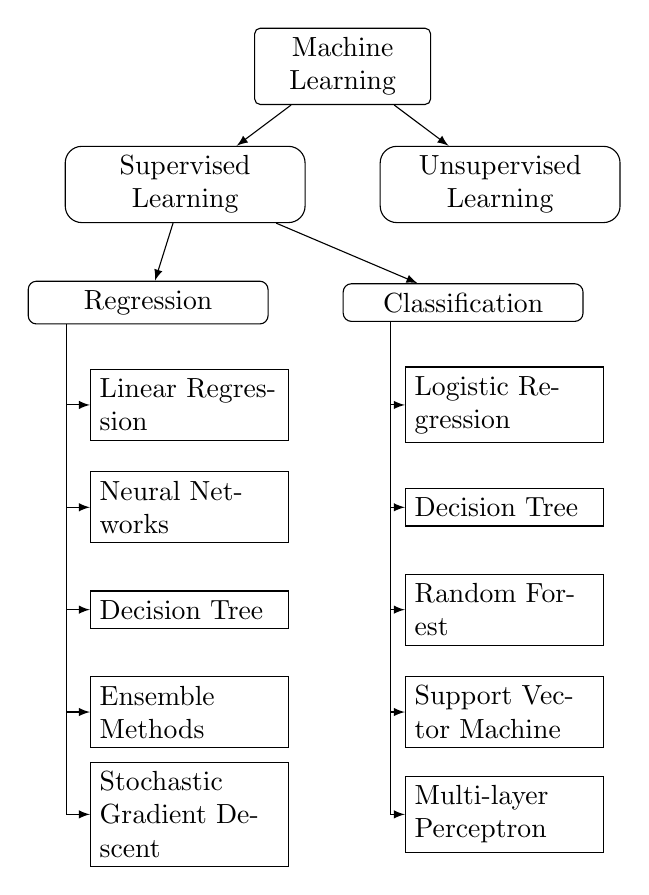
\begin{tikzpicture}[
			level 1/.style={sibling distance=40mm},
			edge from parent/.style={->,draw},
			>=latex]
			
			% root of the the initial tree, level 1
			\node[root] {Machine Learning}
			% The first level, as children of the initial tree
			child {node[level 2] (c3) {Supervised Learning}
				child {node[level 3, anchor=west] (c4) {Regression}}
				child {node[level 3, anchor=west] (c5) {Classification}}}
			child {node[level 2] (c2) {Unsupervised Learning}};
			
			% The second level, relatively positioned nodes
			\begin{scope}[every node/.style={level 4},node distance=1.3cm, auto]
				
				\node [below of = c5, xshift=15pt] (c51) {Logistic Regression};
				\node [below of = c51] (c52) {Decision Tree};
				\node [below of = c52] (c53) {Random Forest};
				\node [below of = c53] (c54) {Support Vector Machine};
				\node [below of = c54] (c55) {Multi-layer Perceptron};
				
				\node [below of = c4, xshift=15pt] (c41) {Linear Regression};
				\node [below of = c41] (c42) {Neural Networks};
				\node [below of = c42] (c43) {Decision Tree};
				\node [below of = c43] (c44) {Ensemble Methods};
				\node [below of = c44] (c45) {Stochastic Gradient Descent};
			\end{scope}
			
			% lines from each level 1 node to every one of its "children"
			\foreach \value in {1,...,5}
			\draw[->] (c4.195) |- (c4\value.west);
			
			\foreach \value in {1,...,5}
			\draw[->] (c5.195) |- (c5\value.west);
		\end{tikzpicture}
	\caption[]{Machine learning classification tree diagram}
	\label{ML Tree Diagram}
	\end{figure}	
	Machine learning is classified into Supervised Learning and Unsupervised Learning along with others like Semi-Supervised Learning, Reinforcement Learning, Multi-task Learning, Ensemble Learning, Neural Networks and Instance-Based Learning \cite{C2}.\\ 
	Unsupervised learning is a form of machine learning technique that unearths obscure patterns or data clusters without the assistance of a human \cite{C4}.\\
	
	In this paper, supervised learning was studied. It is machine learning algorithm that can develop broad patterns and hypotheses by using examples from outside sources to predict the results of incoming examples. The goal of supervised machine learning classification algorithms is to classify data based on existing knowledge (Labelled data) \cite{C3}. Supervised Learning is further categorised into two parts i.e. Regression and Classification.\\
	Regression is frequently used for forecasting and prediction, two areas where machine learning and their application have a lot in common. \\
	
	Supervised classification is one of the functions that so-called intelligent systems carry out most frequently\cite{C7}. The goal of supervised learning is to create a precise model of the distribution of class labels in terms of predictor features. When the values of the predictor characteristics are known but the value of the class label is unknown, the resulting classifier is used to give class labels to the testing cases. In this paper, we focus on the classification of GPU based on memory type (Target variable).\\
	Classification is a data mining technique used to predict data instance group membership\cite{C9}\\
	\begin{figure}[H]
		\resizebox{9cm}{!}{
		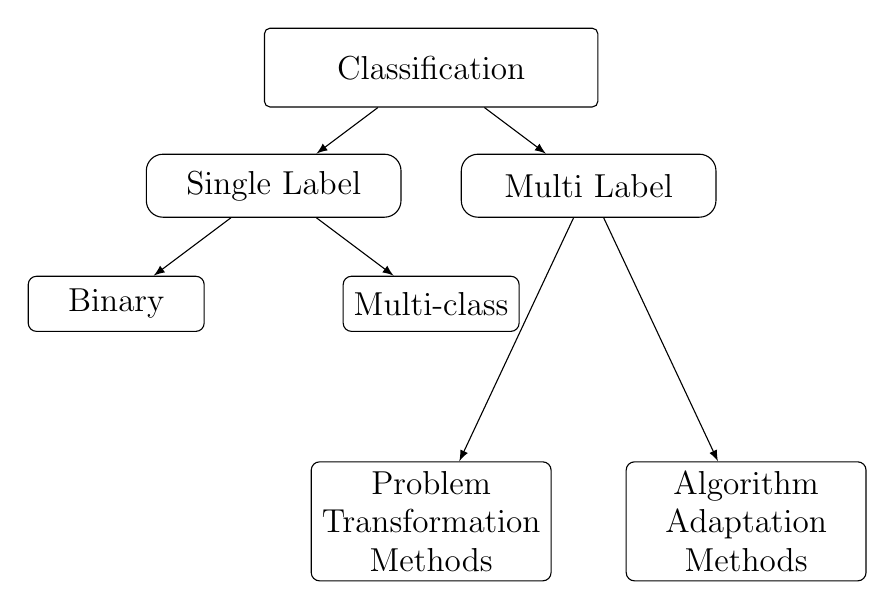
\begin{tikzpicture}[
			level 1/.style={sibling distance=40mm},
			edge from parent/.style={->,draw},
			>=latex]
			
			% root of the the initial tree, level 1
			\node[root,font=\large, text width=4cm, minimum height=1cm] {Classification}
			% The first level, as children of the initial tree
			child {node[level 2, text width=3cm, font=\large,minimum height=0.8cm] (c3) {Single Label}
				child {node[level 3,font=\large,text width=2cm,minimum height=0.7cm] {Binary}}
				child {node[level 3,font=\large,text width=2cm,minimum height=0.7cm] {Multi-class}}}
			child {node[level 2, text width=3cm,font=\large, minimum height=0.8cm] (c2) {Multi Label}
				child {node[level 3, below=2cm,font=\large] {Problem Transformation Methods}}
				child {node[level 3, below=2cm,font=\large] {Algorithm Adaptation Methods}}};
		\end{tikzpicture}
		}
		\caption{Types of classification techniques}
		\label{Classification Tree Diagram}
	\end{figure}

	Most classification problems assign a single class to each example or instance\cite{b1}. However, there are many classification tasks in which each instance can be assigned to one or more classes. This set of problems falls under the category of multi-label classification\cite{C10}. Multi-label classification is further categorised into two types, Problem Transformation Methods and  Algorithm Adaptation Methods.\\ 
	
	Part of single label classification technique, binary classification is a supervised learning algorithm that categorizes new observations into one of two classes\cite{C13}. \\
	A multiclass classification task is a machine learning classification task with more than two classes or outputs\cite{C14}. It assumes that each sample has only one label and employs the Bayes theorem to predict the class of unknown datasets\cite{C14}.\\	
	
	A study presents a network kernel function called Multi-field packet classification, which classifies and routes packets on a GPU using a set of rules\cite{C15}. Another study utilizes a shapelet discovery algorithm for time series classification, which identifies useful subsequences from a set of time series\cite{C16}. The study notes that with recent advancements in high-performance computing techniques, such as GPU, large-scale deep learning models are now possible for machine learning applications\cite{C17}. However, there is a lack of research on CPU classification. To address this gap, the study conducts GPU classification using different types of graphics memory and evaluates and compares three classification algorithms (Random Forest, Support Vector Classification and Decision Tree classifier).
	
\section{Solutions}
	The proposed solution is to use machine learning algorithms to classify Graphics Processing Units based on memory type. This would help to automate the process of product recommendations for technology experts and make it easier to keep track of the ever-demanding technology market. The proposed solution takes advantage of machine learning algorithms such as Random Forest, Decision Tree and Support Vector Machine to classify GPUs based on memory type. The implementation for these algorithm is given below.
	\subsection{Classifiers}
	\subsubsection[H]{Random Forest}
	In 2001, Leo Breiman of the University of California proposed the Random Forest \cite{C26}. It is a classifier composed of a collection of tree-structured classifiers with identically distributed independent random vectors, with each tree casting a unit vote for the most popular class at input $x$\cite{C27}. An upper bound for Random Forests is extracted to get the generalisation error in terms of two parameters exactitude and interdependence of individual classifiers \cite{C25}. \figurename{\ref{Random Forest}} depicts the entire classification process based on the random forest.\\	
	\begin{figure}[H]
		\centerline{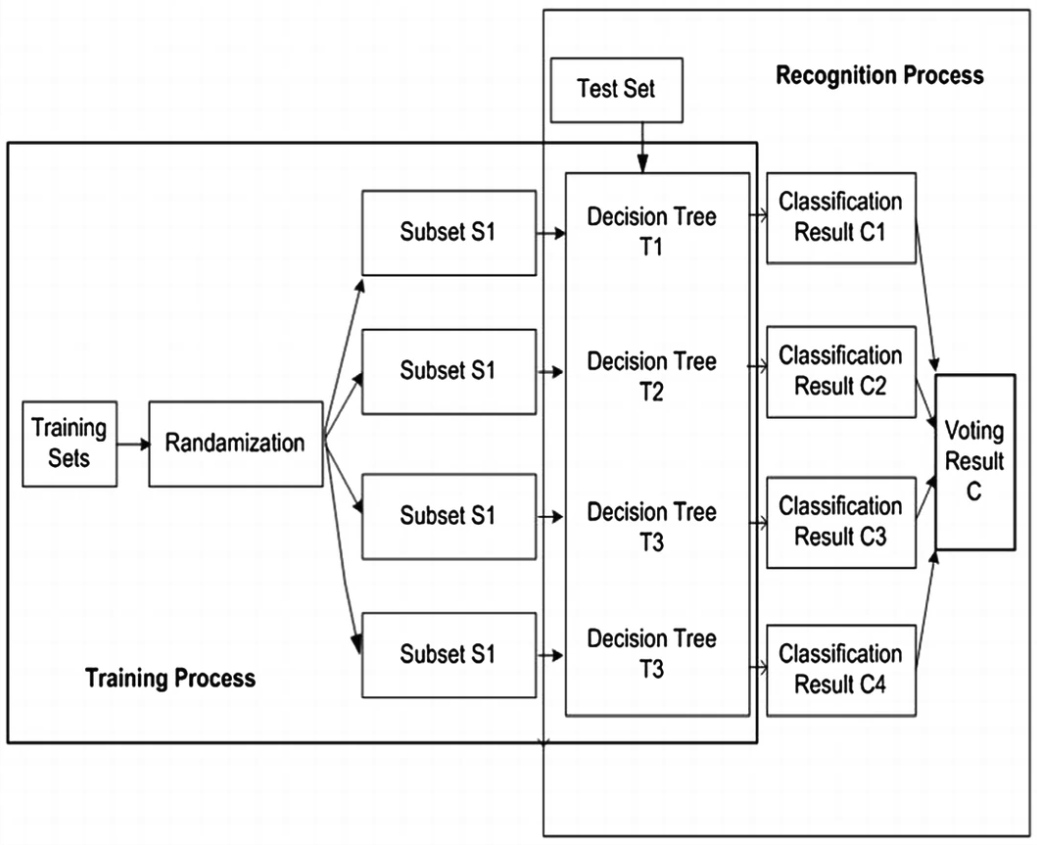
\includegraphics[width=80mm,scale=1]{RandomForest.png}}
		\caption{Conceptual framework of random forest classifier\cite{C24}.}
		\label{Random Forest}
	\end{figure}	
	Random forest is a type of ensemble learning algorithm that builds small decision trees with a limited number of features. The random forest categorises data points with each tree and the average of these decision trees becomes the prediction model.\\	
	\textbf{Formalization:} The algorithm takes a set of elements as input.\\	
	\begin{equation*}
			(N,n,e) \to \frac{1}{n} \sum_{i=1}^{n}f_{n}(x,e) \to f(x) \\ 
	\end{equation*}
	$\text{Where, } N - \text{training data}, e - \text{Entropy}, n - \text{Number of decision trees}$

	\begin{algorithm}[!ht]
		\vspace{1em}
		\KwIn{\small Data set \( N \)}
		\KwOut{\small Find differnent classes of objects}
		
		\vspace{1em}
		
		\SetKwFunction{FMain}{RandomForestClassifier}
		\SetKwProg{Fn}{Function}{:}{}
		\Fn{\FMain{$X$, $y$, $n$, $e$}}
		{
			{
				$DF \leftarrow \phi$\;
			\For{$x \in X$}
			{
					$x_{i} \leftarrowtail BTS(X);$\\
					$f \subset F;$\\
					$d_{i} \leftarrow f_n{}(x,f,e);$\\
					$DF \leftarrow DF \cup d_{i};$\\
			}
		}
			\Return{\( DF ;\)}
		}
		
		\label{Random Forest Algo}
		\vspace{1em}
		\caption{Random forest}%
	\end{algorithm}

	

	\subsubsection[H]{Decision Tree}		
	A decision tree is the most commonly used decision-making tool. To accomplish this, create a decision tree with various branches and leaves. These branches and leaves should represent all of the various aspects of a given situation\cite{C28}. A decision tree functions similarly to a decision support tool. It employs a tree-like graph of decisions and their potential outcomes, such as resource costs, event outcomes and utility. It is one method of displaying an algorithm\cite{C28}. Various types of decision trees can be used depending on the situation and desired outcome.\\	
	\begin{figure}[H]
		\resizebox{9cm}{!}{
			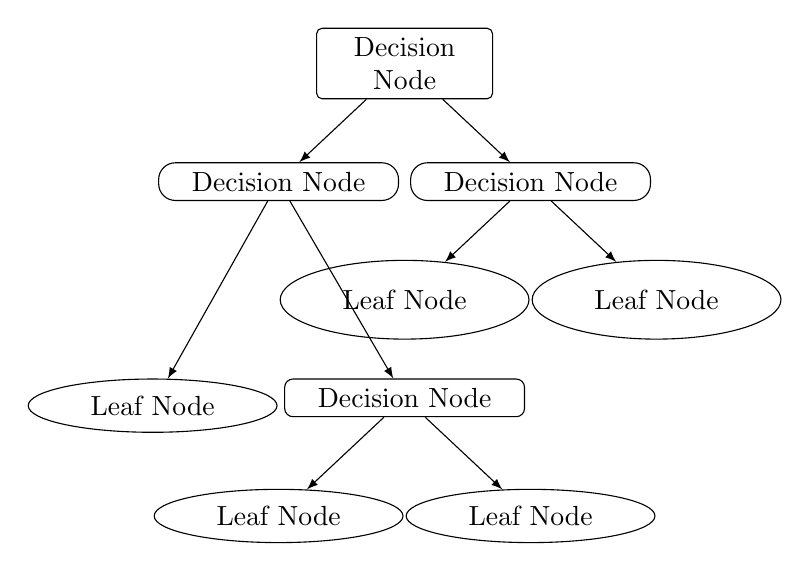
\begin{tikzpicture}[
				level 1/.style={sibling distance=32mm},
				edge from parent/.style={->,draw},
				>=latex]
				\node[root] {Decision Node}
				child {node[level 2] (c3) {Decision Node}
					child {node[round, below=1cm] {Leaf Node}}
					child {node[level 3, below=1cm] {Decision Node}
						child {node[round] {Leaf Node}}
						child {node[round] {Leaf Node}}}}
				child {node[level 2] (c2) {Decision Node}
					child {node[round, minimum height=1cm] {Leaf Node}}
					child {node[round, minimum height=1cm] {Leaf Node}}};				
			\end{tikzpicture}
		}
		\caption[]{Decision tree training flow chart}
		\label{Tree Diagram}
	\end{figure}
	
		A decision tree algorithm is a supervised learning method used for classification and regression problems. The algorithm works by recursively splitting the data into subsets based on the values of input features, creating a tree-like structure. Each internal node of the tree represents a feature and each leaf node represents a class label or a predicted value.
		\begin{algorithm}[!ht]		
			\vspace{1em}
			\KwIn{\small Examples: $E$, Attributes: $A$, Parent Examples: $PE$}
			\KwOut{\small Decision Tree: T}
			\SetKwFunction{FMain}{DecisionTreeClassifier}
			\SetKwProg{Fn}{Function}{:}{}
			\Fn{\FMain{$E$, $A$, $PE$}}
			{
			\KwResult{Decision Tree: $T$}
			\If{$|E| = 0$}{
				\Return{pluralityValue(PE)}
			}
			\If{$|A| = 0$}{
				\Return{pluralityValue(E)}
			}
			\If{$\forall e \in E, e$ classifies the same}{
				\Return{the classification}
			}
			$A' = \operatorname{argmax}_{a \in A} (importance(a, E))$\;
			$T = newTree(root=A')$\;
			\For{$v \in A'$}{
				$exs = \{e \in E | e.A' = v\}$\;
				$subtree = decisionTreeLearning(exs, A - A', E)$\;
				$T.addSubtreeAsBranch(subtree, label=(A', v))$\;
			}
			\Return{ $T$}
		}
			\caption{Decision tree}
		\end{algorithm}		
	\\Where, $E$ represents the set of examples, $A$ represents the set of attributes, $PE$ represents the set of parent examples, $T$ represents the decision tree, $A'$ is the most promising attribute and importance(a, E) is a function to find the importance of attribute an over examples E.\\
	
	\subsubsection{Support Vector Machine}
	
	The C-support vector classification (C-SVC) method is a data mining extension of the SVM (support vector machine) that has many applications in data classification, regression and others\cite{C18}. The letter 'C' in C-SVC stands for the regularisation parameter, which affects the margin of separation between classes. A higher value of C leads to a narrower margin, while a lower value of C leads to a wider margin\cite{C19}.\\
	The implementation is built on top of libsvm. Fit time scales at least quadratically with sample number and may be impractical beyond tens of thousands of samples\footnote{https://scikit-learn.org/stable/modules/generated/sklearn.svm.SVC.html}.\\	
	Support vector machine is a supervised learning algorithm that determines the decision boundary between two classes of objects. It is a linear or non-linear classifier that distinguishes between the two types of data points. It employs the kernel function to determine a decision boundary between data points for non-linear data points.\\
	\textbf{Formalization:} The algorithm take a set of an element as input.\\	
	\begin{equation*}
		(N, K) \rightarrow \sum_{i=1}^{n} \alpha_{i} \ \ y_{i} \ \ K(x_{i}, x) + b \rightarrow f(x)
	\end{equation*}
		Where, $N-$ training data, $K-$ kernel function
	\begin{algorithm}[!ht]
		\vspace{1em}
		\KwIn{\small Data set \( N \)}
		\KwOut{\small Find differnent classes of objects}
		
		\vspace{1em}
		
		\SetKwFunction{FMain}{SVC}
		\SetKwProg{Fn}{Function}{:}{}
		\Fn{\FMain{$X$, $y$, $k$}}
		{
			$V \leftarrow \phi$\;
			\For{$x \in X$}
			{
				$x_{k} = k(X);$\\
				$v= v - x_{k};$\\
				$V \leftarrow V \cup v;$\\
			}
			\Return{\( V ;\)}
		}
		\label{Support Vector Machine}
		\vspace{1em}
		\caption{Support vector machine}%
	\end{algorithm}

	\subsubsection{Performance Metrics}
	A Confusion Matrix and Cross-Validation are both commonly used performance matrices for evaluating the effectiveness of classification algorithms in ML.\\
	\\
	\textit{Confusion matrix:}\\
	A Confusion Matrix is a commonly used performance matrix for classification algorithms. It is a table that is used to compare the predicted values of a model with the actual values and it is particularly useful for classification problems with multiple output classes. The matrix is organized as an N*N table, where N represents the number of output classes. The four different combinations of predicted and actual values are represented in the matrix and are used to calculate other performance metrics such as accuracy, precision, recall and F1-score\cite{C34}.\\
	
	The Confusion matrix typically contains the following four combinations of predicted and actual values:
	\begin{itemize}
	\item True Positives (TP) - the number of observations that are correctly predicted as positive
	\item False Positives (FP) - the number of observations that are incorrectly predicted as positive
	\item True Negatives (TN) - the number of observations that are correctly predicted as negative
	\item False Negatives (FN) - the number of observations that are incorrectly predicted as negative
	\end{itemize}

	These values are used to calculate various metrics such as accuracy, precision, recall and F1-score which gives a holistic view of the performance of the model\cite{C35}.\\
	
	\noindent Accuracy is defined as the ratio of correctly predicted observations to total observations\cite{C35}.
	\begin{equation*}
		Accuracy = \frac{(TP + TN)} {(TP + FP +TN + FN)}
	\end{equation*}
	
	\noindent Precision is defined as the ratio of true positive values to total correctly predicted values \cite{C35}.
	\begin{equation*}
		Precision = \frac{TP}{(TP + FP)}
	\end{equation*}
	
	\noindent The number of correctly predicted values from all positive classes is defined as recall. It is also known as sensitivity\cite{C36}.
	
	\begin{equation*}
		Recall = \frac{TP}{(TP + FP)}
	\end{equation*}
	
	\noindent The F\textsubscript{1} score is the weighted average of precision \& recall\footnote{https://en.wikipedia.org/wiki/F-score}.
	
	\begin{equation*}
		{\displaystyle F_{1}=2{\frac {\mathrm {precision} \cdot \mathrm {recall} }{\mathrm {precision} +\mathrm {recall} }}={\frac {2\mathrm {tp} }{2\mathrm {tp} +\mathrm {fp} +\mathrm {fn} }}}
	\end{equation*}
	\\
	\textit{Cross-validation - StratifiedKFold:}\\
	Cross-validation is a technique that is used to assess the performance of a model by splitting the data into several partitions, training the model on one partition and testing it on the other partition\cite{C37}. This is done multiple times, each time using a different partition for testing and the results are then averaged to give an overall estimate of the model's performance\cite{C37}. \\
	StratifiedKFold is a variation of K-fold cross-validation that ensures each fold has a similar proportion of samples from each class. It was used with 10 folds for better cross-validation and tested 1200+ times to account for variations in execution time.
	
\section{Experiments and Results}
	\noindent \textit{Data Preparation}: A Kaggle dataset named Data Mining UNDIP\footnote{https://www.kaggle.com/code/yukihm/data-mining-undip} was chosen for this classification simulation. It contained a total of  \textbf{2889} samples and \textbf{16} feature, out of which \textbf{5} features were considered to train the models (Dependent Variable - Memory Type and Independent Variables - Memory Size, GPU Clock, Memory Clock, Memory Bus Width), refer to \figurename{\ref{dataset}}. Interpolation was used for generating and filling in missing values in the dataset. The dataset was split into \textbf{80-20\%} for training and testing respectively.
	\begin{figure}[H]{}
	\centerline{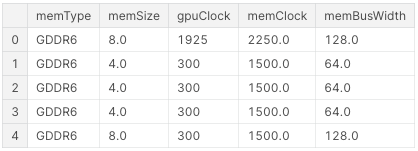
\includegraphics[width=90mm,scale=1]{dataset.png}}
	\caption{Dataset snapshot}
	\label{dataset}
	\end{figure}
	A pearson's corelation was perform to check the corelation between independent variables. It resulted in corelation between all four features which can be verified from the corelation heatmap, refer to \figurename{\ref{DataCorelation}}. For further dataset analysis and visualisation, refer to Appendix \figurename{\ref{DataBarplot}}, \figurename{\ref{DatagpuClockvsmemClock}} and \figurename{\ref{DataPariPlot}}.\\
		\begin{figure}[H]
		\centerline{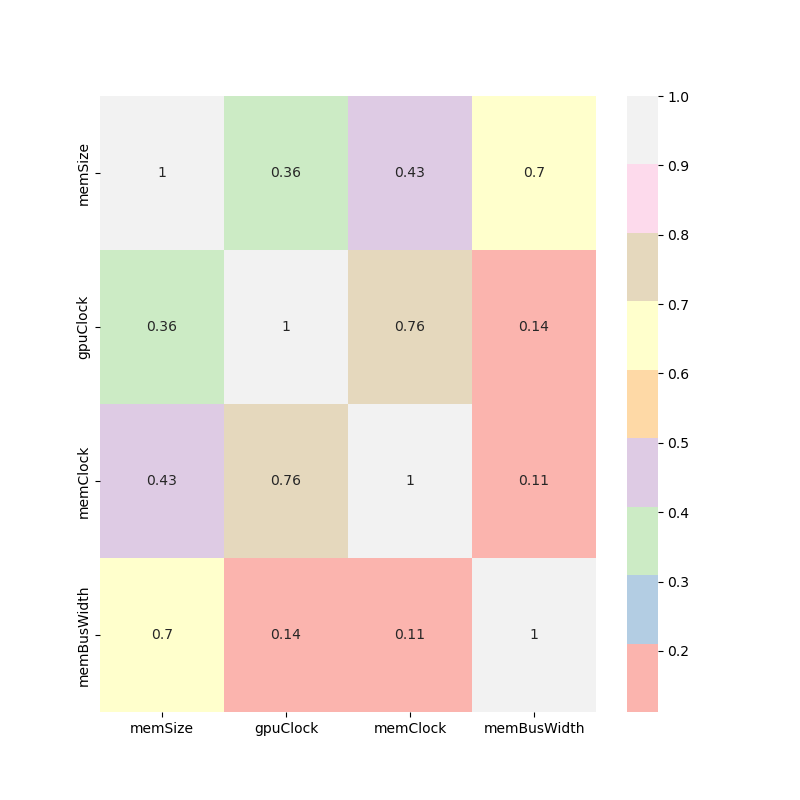
\includegraphics[width=95mm,scale=1]{DataCorelation.png}}
		\caption{Data corelation heatmap}
		\label{DataCorelation}
	\end{figure}
	\noindent \textit{Algorithm Selection}: Three different machine learning algorithms were employed in this study: Random Forest, Decision Tree and Support Vector Machine. These algorithms were chosen as they have been widely used in similar classification tasks and have been shown to produce accurate results.\\\\
	\textit{Algorithm Training}: Each algorithm was trained using the selected features from the dataset and the trained models were used to classify the GPUs based on the memory type.\\\\
	\textit{Evaluation}: The performance for three classifiers (Random Forest, Decision Tree and Support Vector Machine) was evaluated using two techniques, Confusion Matrix and Cross-validation. In cross-validation, along with accuracy, execution time was recorded for over 1200 tests.\\\\
	\textit{Note 1}: The performance evaluation for all three algorithms was measured without parameter optimisation.\\
	\textit{Note 2}: The entire benchmarking was performed using macOS Ventura 13.1 (22C65) running on Apple Macbook Air, Apple M1 (8-Core CPU) and LPDDR4X 16GB RAM.\\
	\subsection{Confusion matrix results}
	In the Confusion Matrix performance evaluation, Accuracy, Precision, Recall and F1 score were recorded on a scale of 0 to 1 (0 being worst and 1 being best). For confusion matrix heatmap plot for all three calssifiers, refer to Appendix \figurename\ref{Confussion matrix heatmap}.\\
		\begin{figure}[H]{}
		\centerline{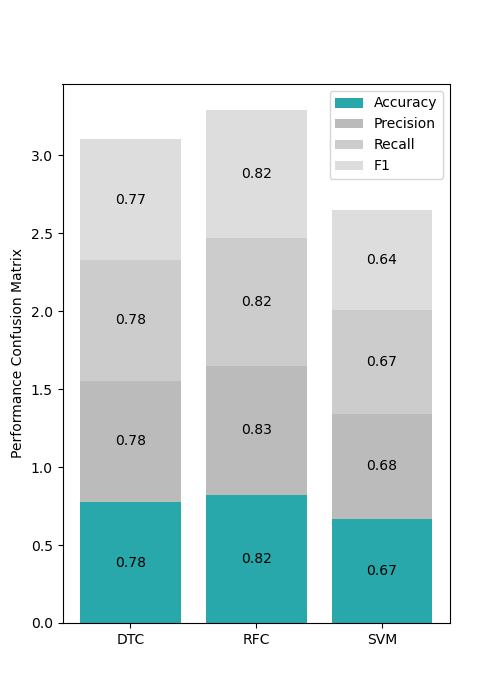
\includegraphics[width=80mm,scale=1]{Performance_CM.png}}
		\caption{Performance based on confusion matrix results}
		\label{Performance_CM}
	\end{figure}
	RFC outperforms other classifiers (DTC and SVM) in each aspect. It has the highest sectional and overall score, refer to \figurename{\ref{Performance_CM}}. However, DTC perform second best and SVM was last.\\
	Clearly from the performance wise Random Forest comes out as the best classification algorithm in comparison with Decision Tree and Support Vector Machine. Refer to \figurename{\ref{Performance_CM}} for confusion matrix results.\\
	Based on these results, it appears that the Random Forest Classifier has the highest accuracy, precision, recall and F1-score among the three algorithms. The Decision Tree Classifier also performed well in terms of accuracy, precision and recall while SVM performed proorly.
 \subsection{Cross-validation results}

		\begin{figure}[H]% ! doesn't do what you think it does
			\centering
			\begin{subfigure}[t]{4cm}
				\centerline{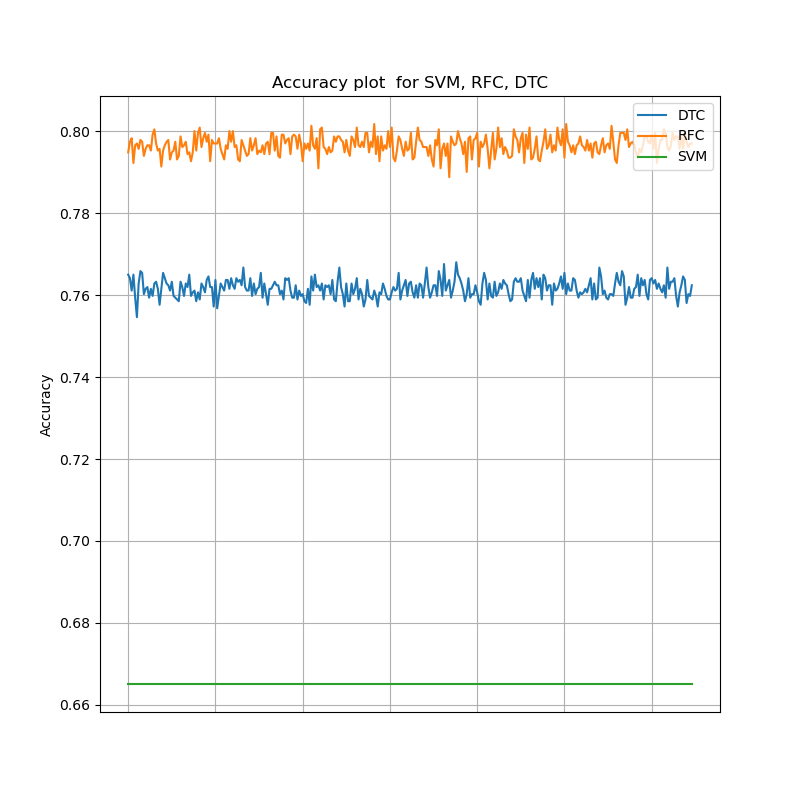
\includegraphics[width=4.7cm,scale=1]{Accuracy Plot.png}}
				\caption{Accuracy plot}
				\label{Accuracy Plot}
			\end{subfigure}\hfil% equal to outside spacing
			\begin{subfigure}[t]{4cm}
				\centerline{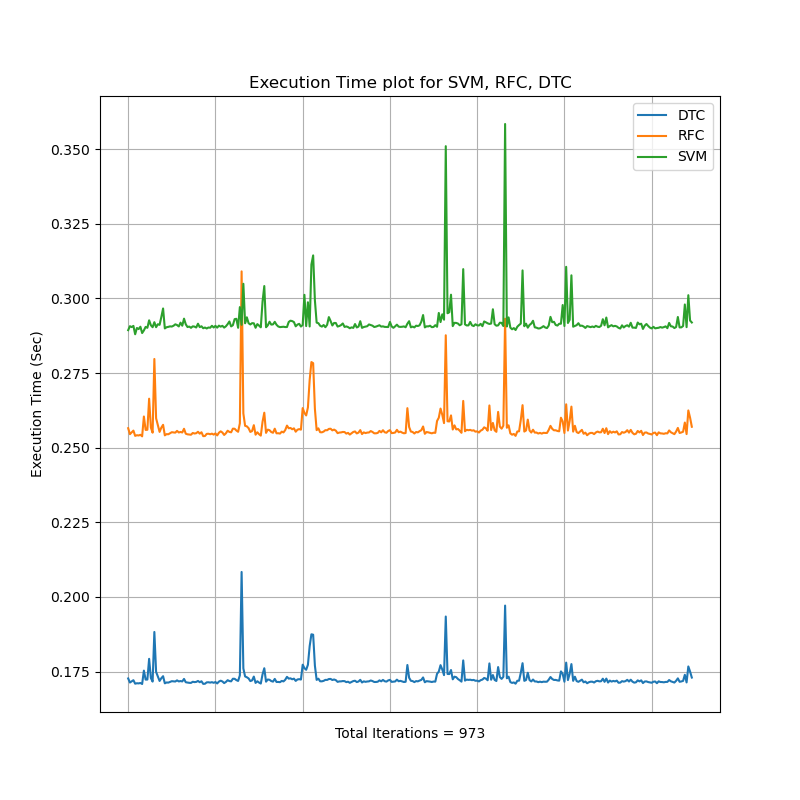
\includegraphics[width=4.7cm,scale=1]{Execution Time Plot.png}}
				\caption{Execution time plot}
				\label{Execution Time Plot}
			\end{subfigure}
		\caption{Accuracy and execution time plot}
		\label{Accuracy and Execution Time Plot}
		\end{figure}	
	\begin{figure}[H]
	\centerline{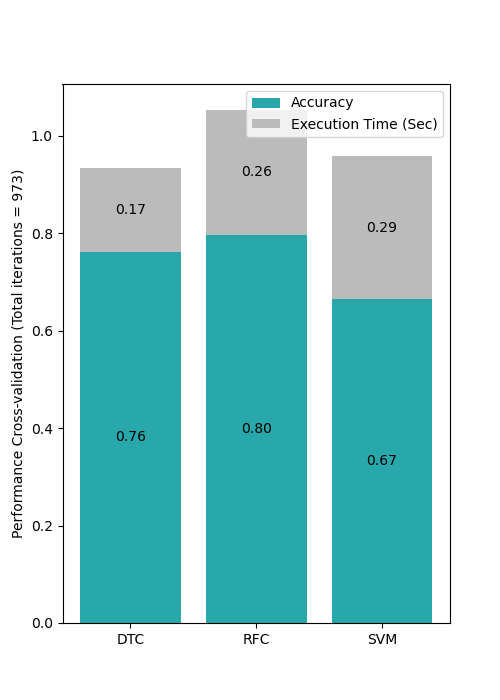
\includegraphics[width=80mm,scale=1]{Performance_CV.png}}
	\caption{Performance based on cross-validation results}
	\label{Performance_CV}
	\end{figure}	
	In terms of execution time, DTC outperformed RFC and SVM by taking the lowest time with \textbf{0.17 Sec}. RFC and SVM performed approximately the same with a of \textbf{0.03 }second difference between them.\\ To see the variations in accuracy and execution time for over 1200 tests, refer to \figurename{\ref{Accuracy and Execution Time Plot}}
	Note: The average was taken from 1261 test results for each classifier.\\
	All three algorithms (DTC, RFC and SVM) showed consistent performance after over 1200 cross-validation tests. SVM was particularly stable with an accuracy of \textbf{0.66}. DTC's accuracy varied between \textbf{0.75} and \textbf{0.77}, while RFC's accuracy ranged from \textbf{0.79} to \textbf{0.81}. Refer to \figurename{\ref{Performance_CV}} for cross-validation results.\\
%	\begin{table}[H]	
%	\begin{center}
%	\begin{tabular}{|c|c|c|c|}
%		\hline
%		\textbf{Classifier Name}&\textbf{Accuracy}  &\textbf{Execution Time} &\textbf{Iterations}   \\ \hline
%		DTC          &0.761        &0.241     &183     \\ \hline
%		RFC          &0.796        &0.358     &183	\\ \hline
%		SVM        	&0.665       &0.366  	 &183     \\ 
%		\hline
%	\end{tabular}
%	\end{center}
%	\caption{Cross-validation results}
%	\label{Results_CV}
%	\end{table}
	\begin{table}[H]	
		\begin{center}
			\begin{tabular}[H]{ |p{1.5cm}|p{0.8cm}|p{0.8cm}|p{0.7cm}|p{0.7cm}|p{0.7cm}|p{0.7cm}|}
				\hline
				\multicolumn{7}{|c|}{\textbf{Combined Results}} \\
				\hline
				\textbf{Classifier}&\textbf{Accu. (CV)} &\textbf{Accu. (CM)} &\textbf{P} &\textbf{R}  &\textbf{F}$_{1}$ &\textbf{ET (sec)}  \\ \hline
															DTC 	&0.761 &0.776 &0.779 &0.776 &0.775 &0.171  \\ \hline
				\rowcolor{pastleyellow} RFC 		&0.796 &0.820 &0.821 &0.820 &0.819 &0.255  \\ \hline
															SVM 	&0.665 &0.666 &0.676 &0.666 &0.639 &0.287   \\ 
				\hline
			\end{tabular}
		\end{center}
		\caption{Overall results}
		\label{Overall Results}
	\end{table}
	The results of the study indicate that the Random Forest Classifier performed the best among the three algorithms considered in this study. The Random Forest Classifier achieved the highest score of \textbf{0.82} in cross-validation (CV) and also had the highest accuracy (Accu.), precision (P), recall (R) and F1-score among the three algorithms as per confusion matrix (CM). Additionally, the Decision Tree Classifier also performed well in terms of accuracy, precision and recall but Random Forest Classifier performed better than DTC. However, the Support Vector Machine had the lowest performance among the three algorithms in all the evaluation metrics. The execution time (ET) for the Random Forest classifier is slightly higher than the Decision Tree Classifier, while Support Vector Machine has the highest execution time among the three classifiers, refer to \figurename{\ref{Overall Results}}.
\section{Summary and Outlook}
	The results of the study showed that the Random Forest algorithm had the highest accuracy in classifying the GPU based on memory type, followed by Decision Tree and Support Vector Machine. The study also evaluated the performance of the algorithms based on precision, recall and F1-score, which are commonly used metrics for evaluating the performance of classification models. However, it should be noted that the study did not include any parameter optimization and the performance could potentially be improved through hypermeter tuning.\\
	
	The study concludes that the proposed classification solution, which utilizes computer processing and machine learning algorithms, can effectively classify GPUs based on memory type. The results of this study can be used to provide more accurate recommendations for technology products and can be extended to other technology products as well. This research can be used as a foundation for further research in the field of technology product classification and it can be useful for consumers, manufacturers and retailers. 
	
	\section*{Appendix}
	\begin{figure}[H]
	\centerline{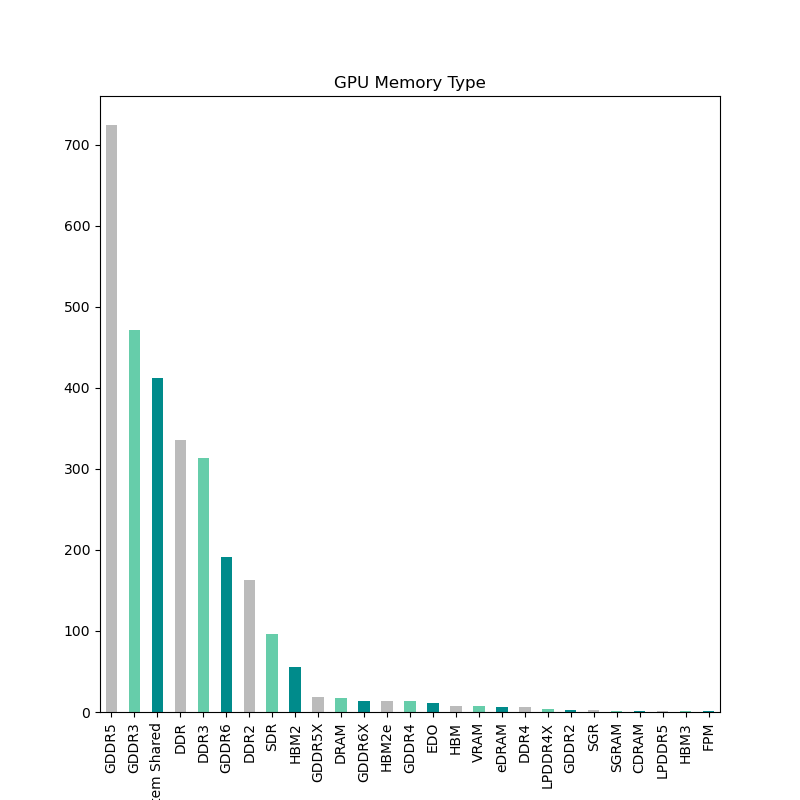
\includegraphics[width=100mm,scale=1]{DataBarplot.png}}
	\caption{Dataset memory type bar plot}
	\label{DataBarplot}
\end{figure}


\begin{figure}[H]
	\centering
	\begin{subfigure}[b]{0.3\textwidth}
		\centering
		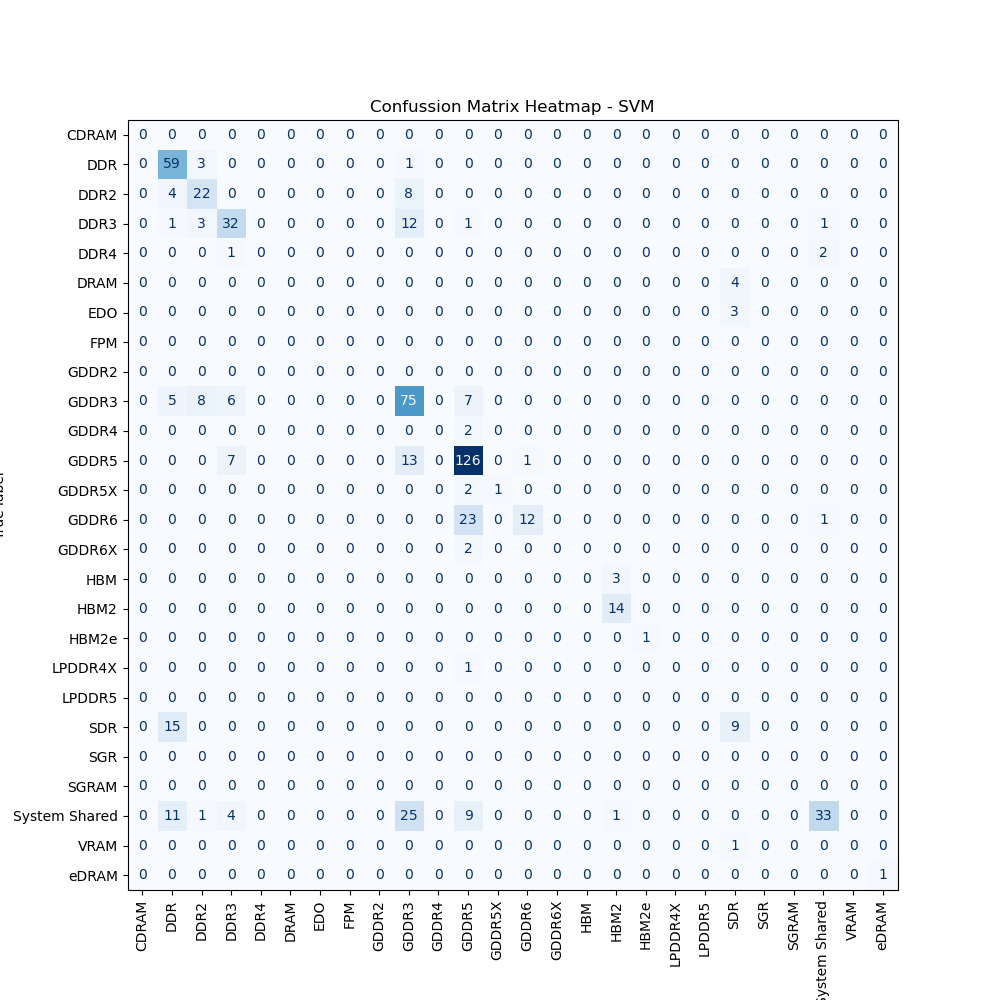
\includegraphics[width=1.3\textwidth]{CM_Heatmap_SVM.png}
		\caption{Heatmap SVM}
		\label{CM_Heatmap_SVM}
	\end{subfigure}
	\hfill
	\begin{subfigure}[b]{0.3\textwidth}
		\centering
		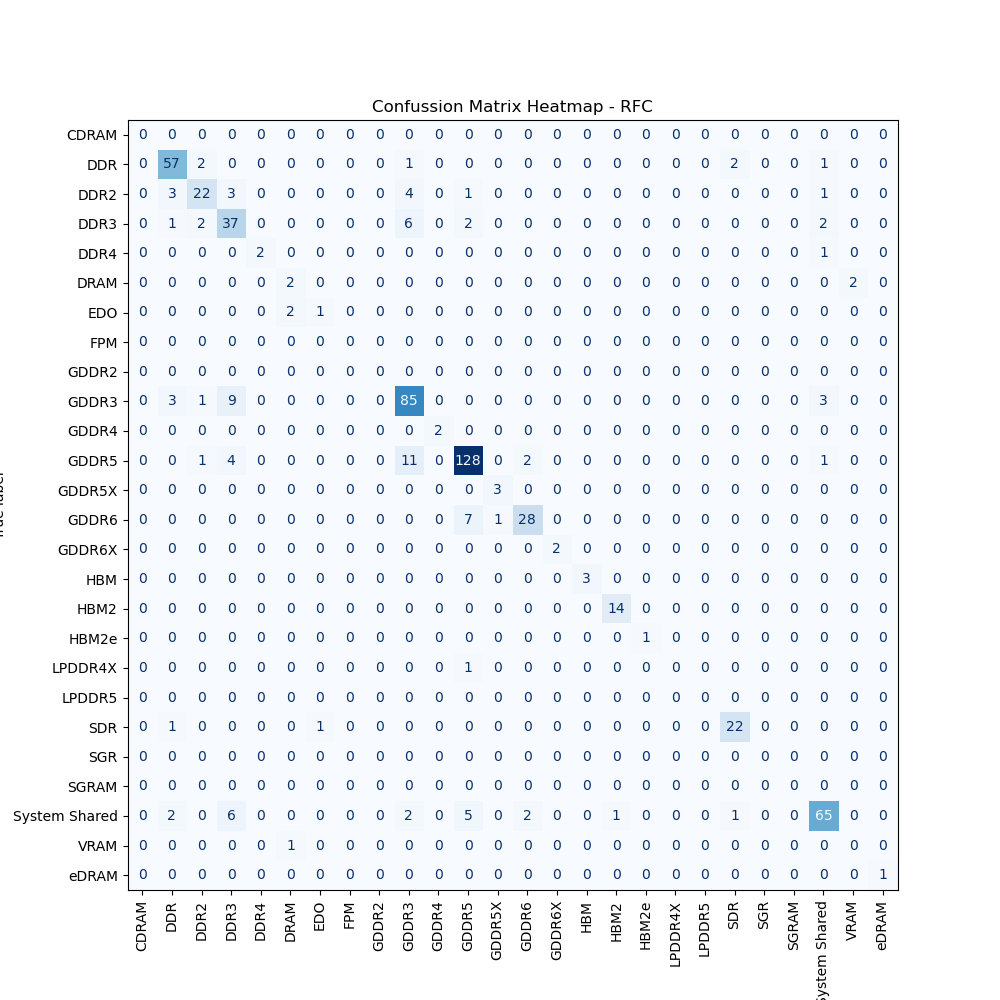
\includegraphics[width=1.3\textwidth]{CM_Heatmap_RFC.png}
		\caption{Heatmap RFC}
		\label{CM_Heatmap_RFC}
	\end{subfigure}
	\hfill
	\begin{subfigure}[b]{0.3\textwidth}
		\centering
		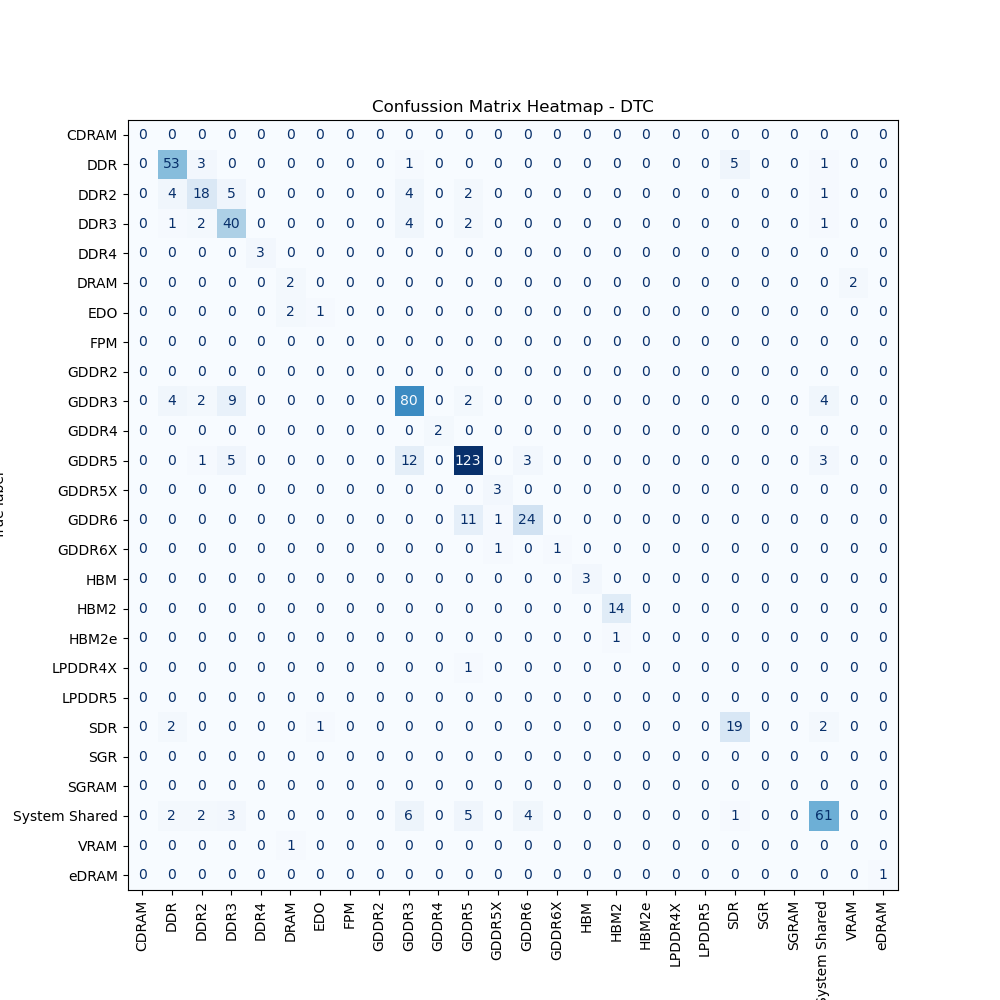
\includegraphics[width=1.3\textwidth]{CM_Heatmap_DTC.png}
		\caption{Heatmap DTC}
		\label{CM_Heatmap_DTC}
	\end{subfigure}
	
	\caption{Confussion matrix heatmap}
	\label{Confussion matrix heatmap}
\end{figure}


\begin{figure}[H]
	\centerline{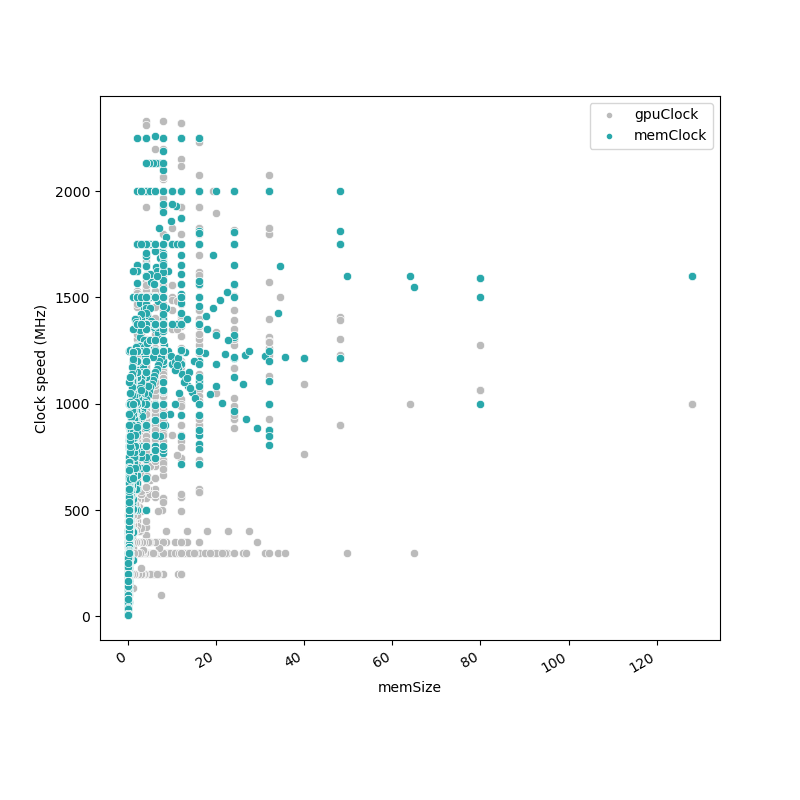
\includegraphics[width=90mm,scale=1]{DatagpuClockvsmemClock.png}}
	\caption{Dataset memSize vs clock speed plot}
	\label{DatagpuClockvsmemClock}
\end{figure}

	\begin{figure}[H]
	\centerline{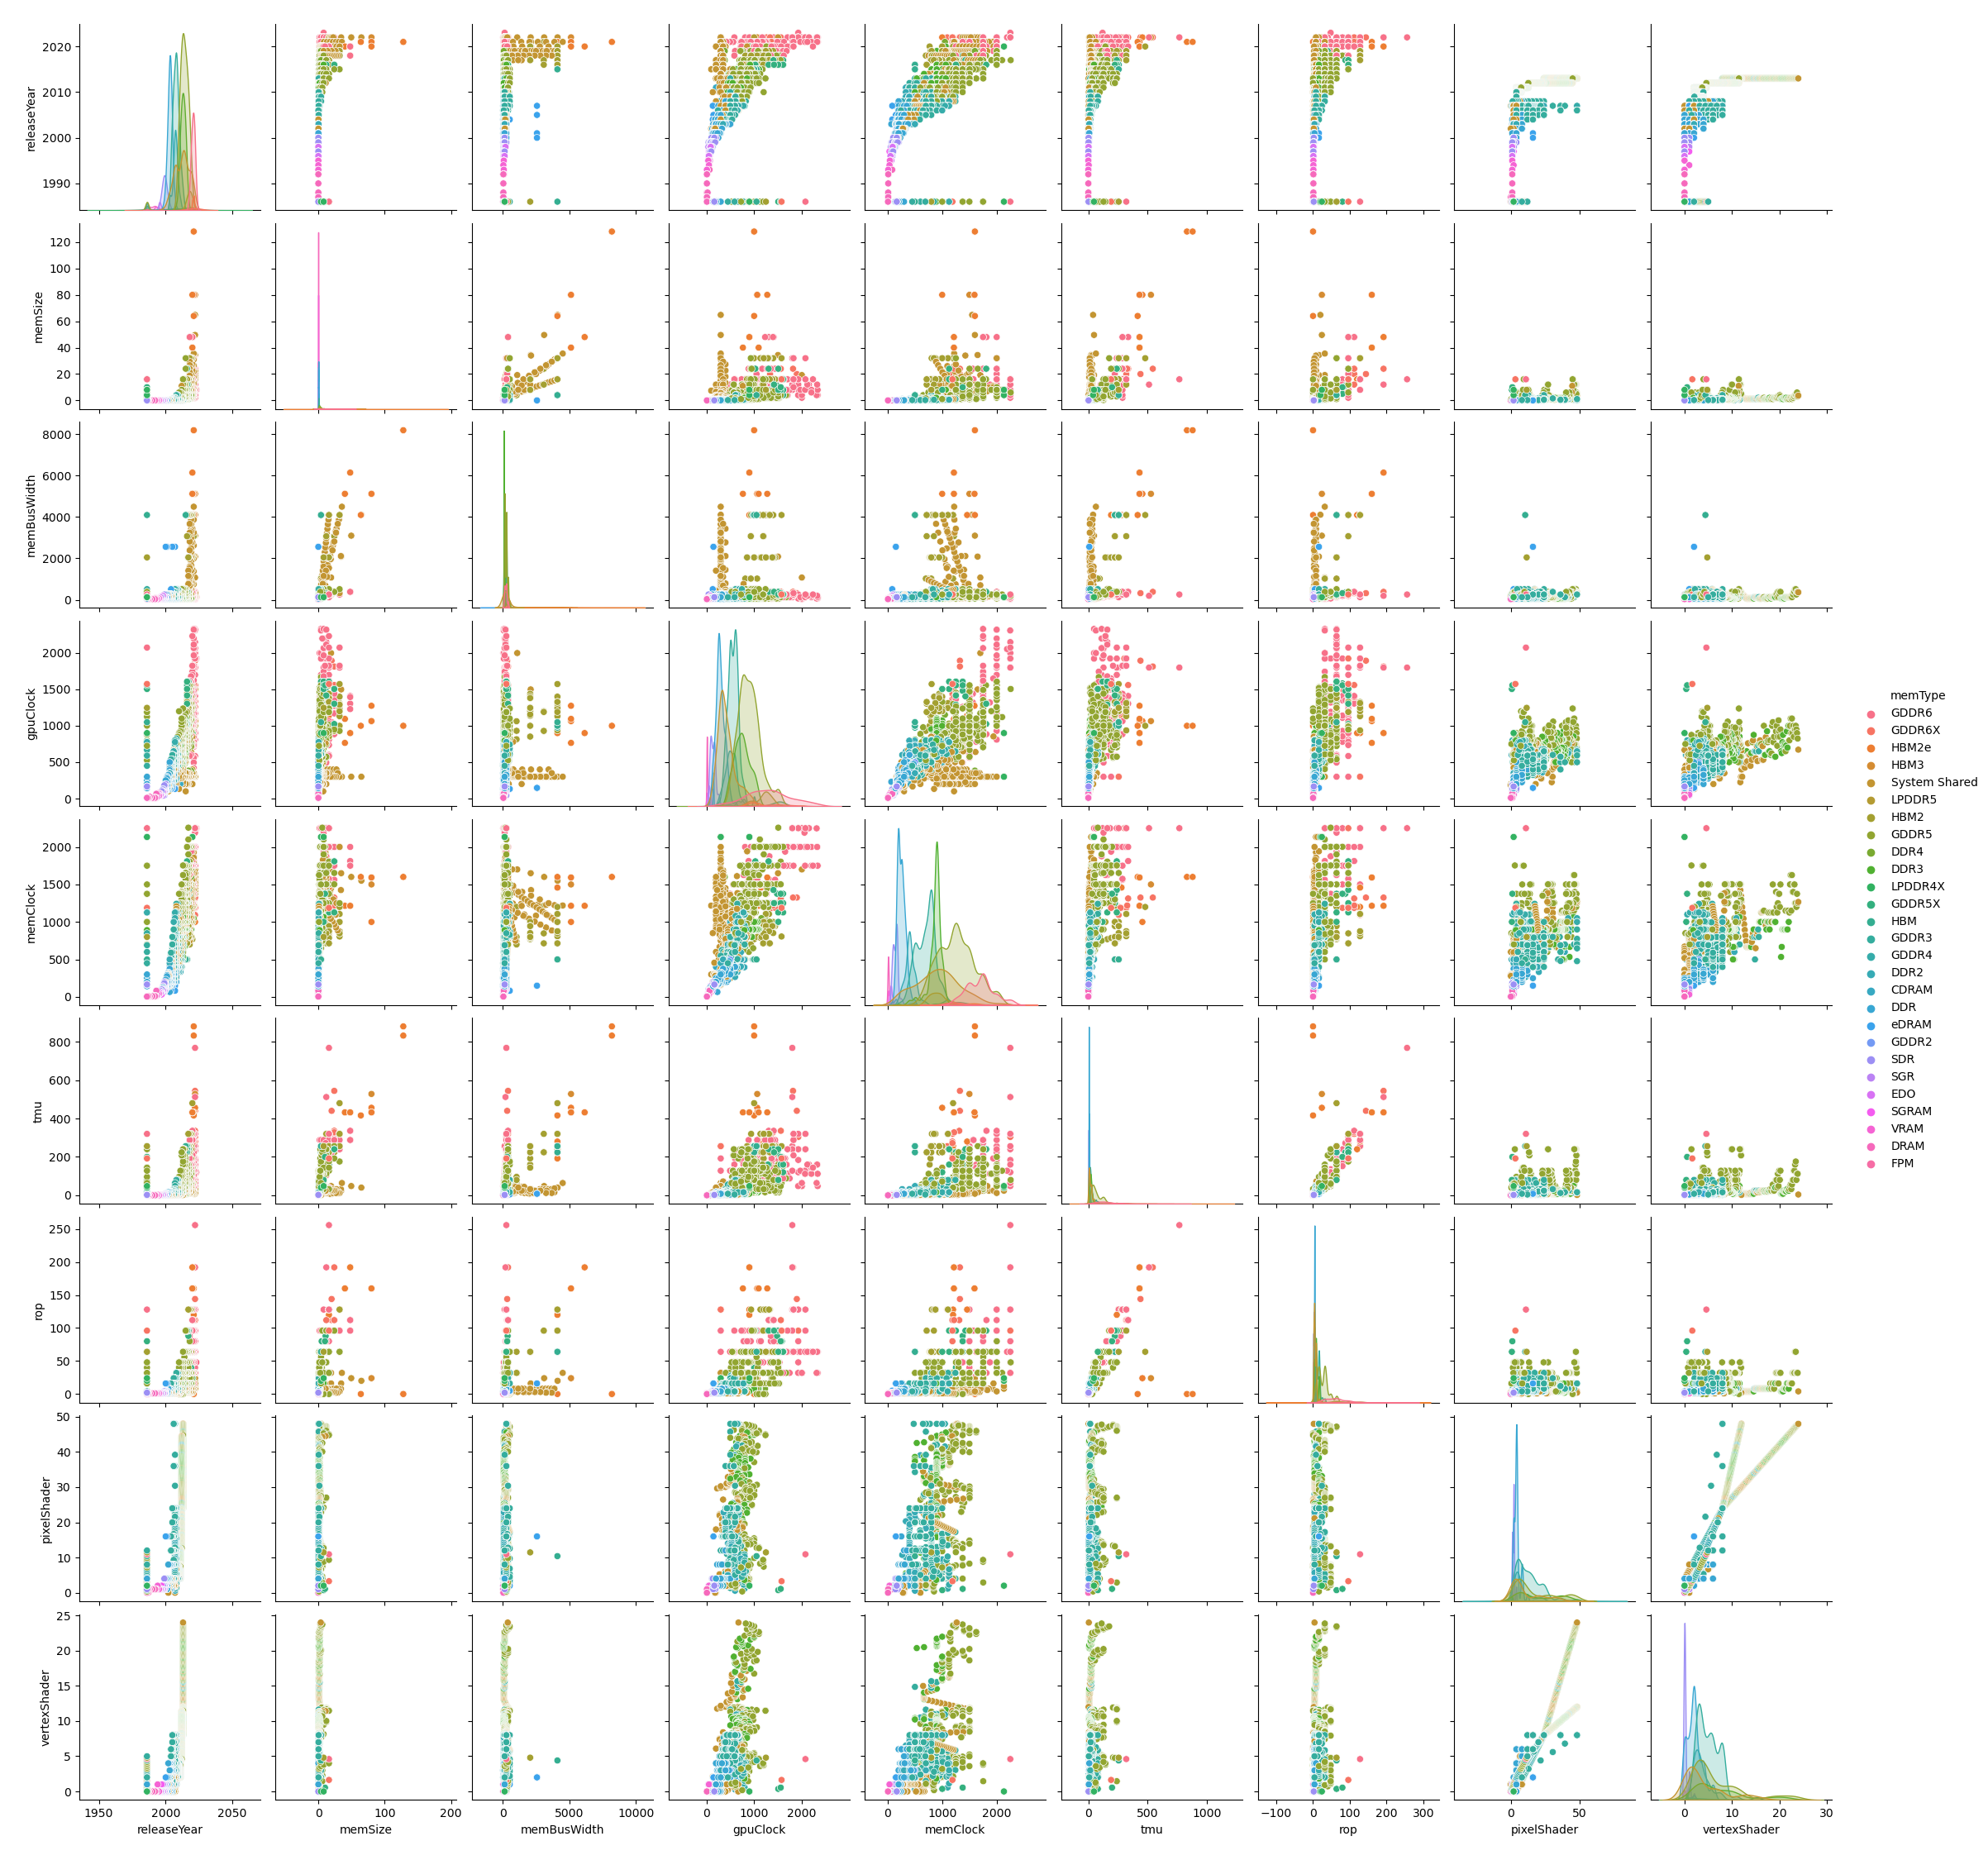
\includegraphics[width=85mm,scale=1]{DataPariPlot.png}}
	\caption{Dataset Hue plot}
	\label{DataPariPlot}
\end{figure}










\begin{thebibliography}{00}

\bibliography{referances.bib}
\nocite{*}
\bibitem{C0}Samuel, A.L., 1959. Some stuies on Machine Learning Using the Game of Checkers. IBM Journal on Research and Development, 3, pp.210-229.	
\bibitem{C01}Mitchell, T.M. and Mitchell, T.M., 1997. Machine learning (Vol. 1, No. 9). New York: McGraw-hill.
\bibitem{C1} Tao Tao, Chen Sun, Zhaoyang Wu, Jian Yang, Jing Wang, Deep Neural Network-Based Prediction and Early Warning of Student Grades and Recommendations for Similar Learning Approaches, Applied Sciences, 10.3390/app12157733, 12, 15, (7733), (2022).
\bibitem{C2}Batta Mahesh Machine Learning Algorithms - A Review International Journal of Science and Research (IJSR) ISSN: 2319-7064 ResearchGate Impact Factor (2018): 0.28 | SJIF (2018): 7.426
\bibitem{C3}A. Singh, N. Thakur and A. Sharma, "A review of supervised machine learning algorithms," 2016 3rd International Conference on Computing for Sustainable Global Development (INDIACom), New Delhi, India, 2016, pp. 1310-1315.
\bibitem{C4}Usama, M., Qadir, J., Raza, A., Arif, H., Yau, K.L.A., Elkhatib, Y., Hussain, A. and Al-Fuqaha, A., 2019. Unsupervised machine learning for networking: Techniques, applications and research challenges. IEEE access, 7, pp.65579-65615.
%\bibitem{C5}Alloghani, M., Al-Jumeily, D., Mustafina, J., Hussain, A. and Aljaaf, A.J., 2020. A systematic review on supervised and unsupervised machine learning algorithms for data science. Supervised and unsupervised learning for data science, pp.3-21.
%\bibitem{C6}J. Wu, C. Liu, W. Cui, and Y. Zhang, "Personalized Collaborative Filtering Recommendation Algorithm based on Linear Regression," in 2019 IEEE International Conference on Power Data Science (ICPDS), 2019, pp. 139-142.
\bibitem{C7}Kotsiantis, S.B., Zaharakis, I. and Pintelas, P., 2007. Supervised machine learning: A review of classification techniques. Emerging artificial intelligence applications in computer engineering, 160(1), pp.3-24.
%\bibitem{C8}Acid S and de Campos LM (2003). Searching for Bayesian network structures in the space of restricted acyclic partially directed graphs. J Artif Intell Res 18: 445–490
\bibitem{b1}AMROUCHE, M.I., CHOUTRI, A.D. and BOUJEBBOUR, K., 2020. Multi-Label Classification of Social Networks’ Users Based on Services (Doctoral dissertation).

\bibitem{C9}Kesavaraj, G. and Sukumaran, S., 2013, July. A study on classification techniques in data mining. In 2013 fourth international conference on computing, communications and networking technologies (ICCCNT) (pp. 1-7). IEEE.
\bibitem{C10}de Carvalho, A.C. and Freitas, A.A., 2009. A tutorial on multi-label classification techniques. Foundations of computational intelligence volume 5, pp.177-195.
%\bibitem{C11}Cherman, E.A., Monard, M.C. and Metz, J., 2011. Multi-label problem transformation methods: a case study. CLEI Electronic Journal, 14(1), pp.4-4.
%\bibitem{C12}Zhang, J., Chen, W.N., Zhan, Z.H., Yu, W.J., Li, Y.L., Chen, N. and Zhou, Q., 2012. A survey on algorithm adaptation in evolutionary computation. Frontiers of Electrical and Electronic Engineering, 7(1), pp.16-31.
\bibitem{C13}Bellinger, C., Sharma, S. and Japkowicz, N., 2012, December. One-class versus binary classification: Which and when?. In 2012 11th international conference on machine learning and applications (Vol. 2, pp. 102-106). IEEE.
\bibitem{C14}Aly, M., 2005. Survey on multiclass classification methods. Neural Netw, 19(1), p.9.
\bibitem{C15}Zhou, S., Singapura, S.G. and Prasanna, V.K., 2014, September. High-performance packet classification on GPU. In 2014 IEEE High Performance Extreme Computing Conference (HPEC) (pp. 1-6). IEEE.
\bibitem{C16}Chang, K.W., Deka, B., Hwu, W.M.W. and Roth, D., 2012, December. Efficient pattern-based time series classification on GPU. In 2012 IEEE 12th International Conference on Data Mining (pp. 131-140). IEEE.
\bibitem{C17}Zhang, Q., Bai, C., Liu, Z., Yang, L.T., Yu, H., Zhao, J. and Yuan, H., 2020. A GPU-based residual network for medical image classification in smart medicine. Information Sciences, 536, pp.91-100.
\bibitem{C18}D. Rahmawati and Y. -P. Huang, "Using C-support vector classification to forecast dengue fever epidemics in Taiwan," 2016 International Conference on System Science and Engineering (ICSSE), Puli, Taiwan, 2016, pp. 1-4, doi: 10.1109/ICSSE.2016.7551552.
\bibitem{C19}Novakovic, J. and Veljovic, A., 2011, September. C-support vector classification: Selection of kernel and parameters in medical diagnosis. In 2011 IEEE 9th international symposium on intelligent systems and informatics (pp. 465-470). IEEE.
%\bibitem{C20}Boser, B.E., Guyon, I.M. and Vapnik, V.N., 1992, July. A training algorithm for optimal margin classifiers. In Proceedings of the fifth annual workshop on Computational learning theory (pp. 144-152).
%\bibitem{C21}Cortes, C. and Vapnik, V., 1995. Support-vector networks. Machine learning, 20(3), pp.273-297.
%\bibitem{C22}Chang, C.C. and Lin, C.J., 2011. LIBSVM: a library for support vector machines. ACM transactions on intelligent systems and technology (TIST), 2(3), pp.1-27.
%\bibitem{C23}Vapnik, V., 1998. Statistical learning theory new york. NY: Wiley, 1(2), p.3.
\bibitem{C24}Parmar, A., Katariya, R. and Patel, V., 2019. A review on random forest: An ensemble classifier. In International Conference on Intelligent Data Communication Technologies and Internet of Things (ICICI) 2018 (pp. 758-763). Springer International Publishing.
\bibitem{C25}Yigin, B.O., Algin, O. and Saygili, G., 2020. Comparison of morphometric parameters in prediction of hydrocephalus using random forests. Computers in Biology and Medicine, 116, p.103547.
\bibitem{C26}Breiman, L., 2001. Random forests. Machine learning, 45(1), pp.5-32.
\bibitem{C27}Reis, I., Baron, D. and Shahaf, S., 2018. Probabilistic random forest: A machine learning algorithm for noisy data sets. The Astronomical Journal, 157(1), p.16.
\bibitem{C28}Navada, A., Ansari, A.N., Patil, S. and Sonkamble, B.A., 2011, June. Overview of use of decision tree algorithms in machine learning. In 2011 IEEE control and system graduate research colloquium (pp. 37-42). IEEE.
%\bibitem{C29}Kumar, G.K., Viswanath, P. and Rao, A.A., 2016. Ensemble of randomized soft decision trees for robust classification. Sādhanā, 41(3), pp.273-282.
%\bibitem{C30}Li, Y., Jiang, Z.L., Yao, L., Wang, X., Yiu, S.M. and Huang, Z., 2019. Outsourced privacy-preserving C4. 5 decision tree algorithm over horizontally and vertically partitioned dataset among multiple parties. Cluster Computing, 22(1), pp.1581-1593.
%\bibitem{C31}Singh, S. and Gupta, P., 2014. Comparative study ID3, cart and C4. 5 decision tree algorithm: a survey. International Journal of Advanced Information Science and Technology (IJAIST), 27(27), pp.97-103.
%\bibitem{C32}Band, S.S., Janizadeh, S., Saha, S., Mukherjee, K., Bozchaloei, S.K., Cerdà, A., Shokri, M. and Mosavi, A., 2020. Evaluating the efficiency of different regression, decision tree, and bayesian machine learning algorithms in spatial piping erosion susceptibility using ALOS/PALSAR Data. Land, 9(10), p.346.
%\bibitem{C33}Sarker, I.H., Colman, A., Han, J., Khan, A.I., Abushark, Y.B. and Salah, K., 2020. Behavdt: a behavioral decision tree learning to build user-centric context-aware predictive model. Mobile Networks and Applications, 25(3), pp.1151-1161.
\bibitem{C34}Patel, H.H. and Prajapati, P., 2018. Study and analysis of decision tree based classification algorithms. International Journal of Computer Sciences and Engineering, 6(10), pp.74-78.
\bibitem{C35}Farnaaz, N. and Jabbar, M.A., 2016. Random forest modeling for network intrusion detection system. Procedia Computer Science, 89, pp.213-217.
\bibitem{C36}Azar, A.T., Elshazly, H.I., Hassanien, A.E. and Elkorany, A.M., 2014. A random forest classifier for lymph diseases. Computer methods and programs in biomedicine, 113(2), pp.465-473.
\bibitem{C37}Artur, M., 2021. Review the performance of the Bernoulli Naïve Bayes Classifier in Intrusion Detection Systems using Recursive Feature Elimination with Cross-validated selection of the best number of features. Procedia Computer Science, 190, pp.564-570.
\end{thebibliography}


\end{document}
